\documentclass[12pt,oneside,openany,a4paper,%..... Layout
               afrikaans, english,%.............. Global language selection
               ]{memoir}

 \usepackage[masters-t,%.......................... Master thesis
             goldenblock,%........................ A5 type block (or a5block or wide)
            ]{usthesis}%.......................... US thesis style with memoir

%
% PLEASE read the USthesis documentation for the class options
% and how to set line and paragraph spacing
%
\OnehalfSpacing

%==== Language setup ================================================
 \usepackage[latin1]{inputenc}%................... Recognizes ê, ë, etc
 \usepackage{babel}%.............................. Language setup

%==== Math setup ====================================================
 \usepackage{amsmath}%............................ Advanced math (before fonts)
 %\usepackage{amssymb}%............................ AMS Symbol fonts

%==== Font setup (default is Computer Modern) =======================
 \usepackage[T1]{fontenc}%........................ Type 1 fonts
 %\usepackage{fourier}
 \usepackage{textcomp}%........................... Additional text character
 \usepackage{bm}%................................. Bold math symbols (after fonts)

%==== Ref's, Bib's and Nomencl ======================================
% \usepackage{usnomencl}%......... List of symbols (in usthesis pack)
% \usepackage{usbib}%............. Bibliography    (in usthesis pack)
%    \bibliographystyle{usmeg-a}
%    \renewcommand\bibfont{\small}
%
%    %% For usmeg-a, the bib is a list of references. If you
%    %% are using usmeg-n comment out the following lines
%    \addto{\captionsafrikaans}{\renewcommand{\bibname}{Lys van Verwysings}}
%    \addto{\captionsenglish}{\renewcommand{\bibname}{List of References}}
    
%=== Biber Commands (USER DEFINED)===================================

\usepackage{csquotes}% Recommended

\usepackage[backend=biber,style=authoryear,uniquename=false]{biblatex}

\addbibresource[]{bibliography/USbib-sample.bib}%...this must point to your bib-file (Syntax for version >= 1.2 of biber engine).
    
%==== Graphics and Color ============================================
\usepackage{graphicx}%........................... Graphicx loaded in usthesis
\usepackage{color}%.............................. Color setup
\usepackage{eso-pic}%............................ Shipout commands for watermark
    \newcommand*{\WaterMark}[2][0.15\paperwidth]{%
        \AddToShipoutPicture*{\AtTextCenter{%
                \parbox[c]{0pt}{\makebox[0pt][c]{%
                    \includegraphics[width=#1]{#2}}}}}}

%==== Local Defs ====================================================
\makeatletter

\usepackage{url}
\usepackage{hyperref}

%
% Please insert user defined commands here
% and NOT in the document itself!
% You might want to do things that require additional packages and then you list the packages here.

\makeatother

%=== Tables =====================================================
\usepackage{booktabs}
%\usepackage{pdflscape}
%\usepackage{longtable}
%\usepackage{tabularx}
%\usepackage{ltablex} 
%\usepackage{lipsum}

\usepackage{float} %...this makes sure that tables don't get repositioned when you use the appropriate command in table.
\restylefloat{table}

%==== TITLE PAGE ====================================================
\title{\bfseries
       \AorE{%-- Afrikaans ------------------------------------------
             Jou Ongelooflike Tesis Titel:\\ En Sub-Titel\\[1ex]
             \normalfont\small\itshape
             (``Your Incredible Thesis Title:\\ And Sub-Title'')
            }{%-- English -------------------------------------------
             Your Incredible Thesis Title:\\ And Sub-Title
            }}

\author{H.\ Wiehahn}{Helena Wiehahn}

\degree{\AorE{MPhil (IKB)}{MPhil (IKM)}}
       {\AorE{Magister in die Wysbegeerte (Informasie en Kennisbestuur)}
             {Master of Philosophy (Information and Knowledge Management)}}

\address{\AorE{%-- Afrikaans ----------------------------------------
        Departement Inligtingwetenskap,\\
        Universiteit van Stellenbosch,\\
        Privaatsak X1, Matieland 7602, Suid Afrika.%
             }{%-- English ------------------------------------------
        Department of Information Science,\\
        University of Stellenbosch,\\
        Private Bag X1, Matieland 7602, South Africa.
             }}

\faculty{\AorE{Fakulteit Lettere en Sosiale Wetenskappe}%
              {Faculty of Arts and Social Sciences}}

\supervisor{Dr.\ Paul Louis\ Iske}
%\cosupervisor{}

\setdate{09}{2020}

%\Sponsorship Disclaimer
%\SetSponsor{The financial assistance of the National Research Foundation (NRF) towards this research is hereby acknowledged. Opinions expressed and conclusions arrived at, are those of the author and are not necessarily to be attributed to the NRF.}


%====================================================================
%     MAIN DOCUMENT
%====================================================================
\maxsecnumdepth{subsubsection}
\maxtocdepth{section}

\begin{document}

%==== Front matter ==================================================
 \frontmatter
 \WaterMark{UScrest-WM}
 \TitlePage

 \DeclarationDate{2020/09/01}
 \DeclarationPage

 \begin{abstract}[english]%===================================================
Here you write a summary of your amazing thesis of less than 500 words.
\end{abstract}


\begin{abstract}[afrikaans]%=================================================
Hier skryf jy 'n Afrikaanse opsomming van minder as 500 woorde.
\end{abstract}


%\chapter{Acknowledgements}%==================================================
%
%I would like to express my sincere gratitude to the following people
%and organisations ...
%This is uncommented and compiled only for the final copy and not for the exam.
%
%\chapter{Dedications}%=======================================================
% \vfill
% \begin{Afr}
% \begin{center}\itshape
%    Hierdie tesis word opgedra aan ...
% \end{center}
% \end{Afr}
% \vfill
% \clearpage

%===========================================================
\endinput


 \tableofcontents
 \clearpage

 \setcounter{lofdepth}{2}
 \listoffigures
 \clearpage

 \listoftables
 \clearpage

% \include{frontmatter/Nomencl}

%==== Main document =================================================
\mainmatter
   \setsecnumdepth{subsubsection}
%   \numberwithin{equation}{section}
%   \numberwithin{figure}{chapter}
%   \numberwithin{table}{chapter}

\chapter{Introduction}
\label{chp:intro}


%%%%%%%%%%%%%%%%%%%%%%%%%%%%%%%%%%%%%%%%%%%%%%%%%%%%%%%%%%%%%%%%%%%%%%%
\section{Background}

Here you write your amazing text.\footnote{You include footnotes like this.} With examples of two types of citations. Some citations happen in parenthesis, for example \parencite[215]{Abma2000} , whilst others are cited in text, such as \textcite[4]{Ancora2012} said that sometimes you want to cite multiple authors at one point, which you do like this \parencite{Czarniawska2000, Weick1995}.

In a later article \parencite[410-413]{Weick2005} the properties are called ``distinctive features'' of sensemaking. 
Note how quotations marks look in TeX, especially the opening ones that can be found near Z on your keyboard and the closing ones that are \emph{TWO} individual ones found near your Return key (and now you know how to make things italics with the emph-command).

\subsection{Next level heading}

Yet more boring text to write and read. You have to write 100-120 pages, but no more than 140. Anything under 100 pages of text is likely too short.

\subsubsection{Third level heading}
At a push you might need even another level down, but think carefully about third level subheadings.

\subsubsection{Another third level heading}
Remember that if you go down a level, the level must always have at least one partner on the same level, otherwise why did you need to go down a level?

\subsection{How to do tables}

Another thing you might want to do is to include a table. This is the only really difficult thing in LaTeX and I propose that you use \url{https://www.tablesgenerator.com/latex_tables} and making your tables in excel, save them as CSV-files and then open them on that site and generate the code there, copy and paste it back in your text. Remember to use the caption and booktabs options for nice looking tables.\footnote{And now you also know how to insert URLs in the text.} 

%%% One can add the option [H] to the table generated, which ensures the table is placed always below the text above. If you leave the option open, then the software decides where to place it best. Usually the default is good enough.
%Possible values are: 
%h (here) - same location
%t (top) - top of page
%b (bottom) - bottom of page
%p (page) - on an extra page
%! (override) - will force the specified location when written behind a value as in [h!]

\begin{table}[h]
\centering
\begin{tabular}{@{}lll@{}}
\toprule
\textbf{SECI} & Tacit           & Explicit        \\ \midrule
Tacit         & Socialization   & Externalization \\
Explicit      & Internalization & Combination     \\ \bottomrule
\end{tabular}
\caption{Nonaka's SECI-model}
\label{tab:seci}
\end{table}

Here you simply continue writing your text. The labels command after sections, tables, or figures and so on can be used for cross-references, like Table \ref{tab:seci} shows the knowledge conversion processes.

\subsection{How to make lists}

You may for instance think that you need to make a list. Such a list can be either bulleted.

\begin{itemize}
	\item apples
	\item oranges
	\item pears
\end{itemize}

Alternatively a list may be numbered like the one here:

\begin{enumerate}
	\item dogs
	\item cats
	\item hamsters
\end{enumerate}

But remember that writing paragraphs are always better than writing lists, because paragraphs contain arguments with reasons, whilst lists only describe. Therefore please do not overuse the list function.

\subsection{How to include figures}

Make sure that you have the figure saved in a format that autoscales easily and in the appropriate folder called ``figs''. Then you include it with the following commands.

\begin{figure}[h]
  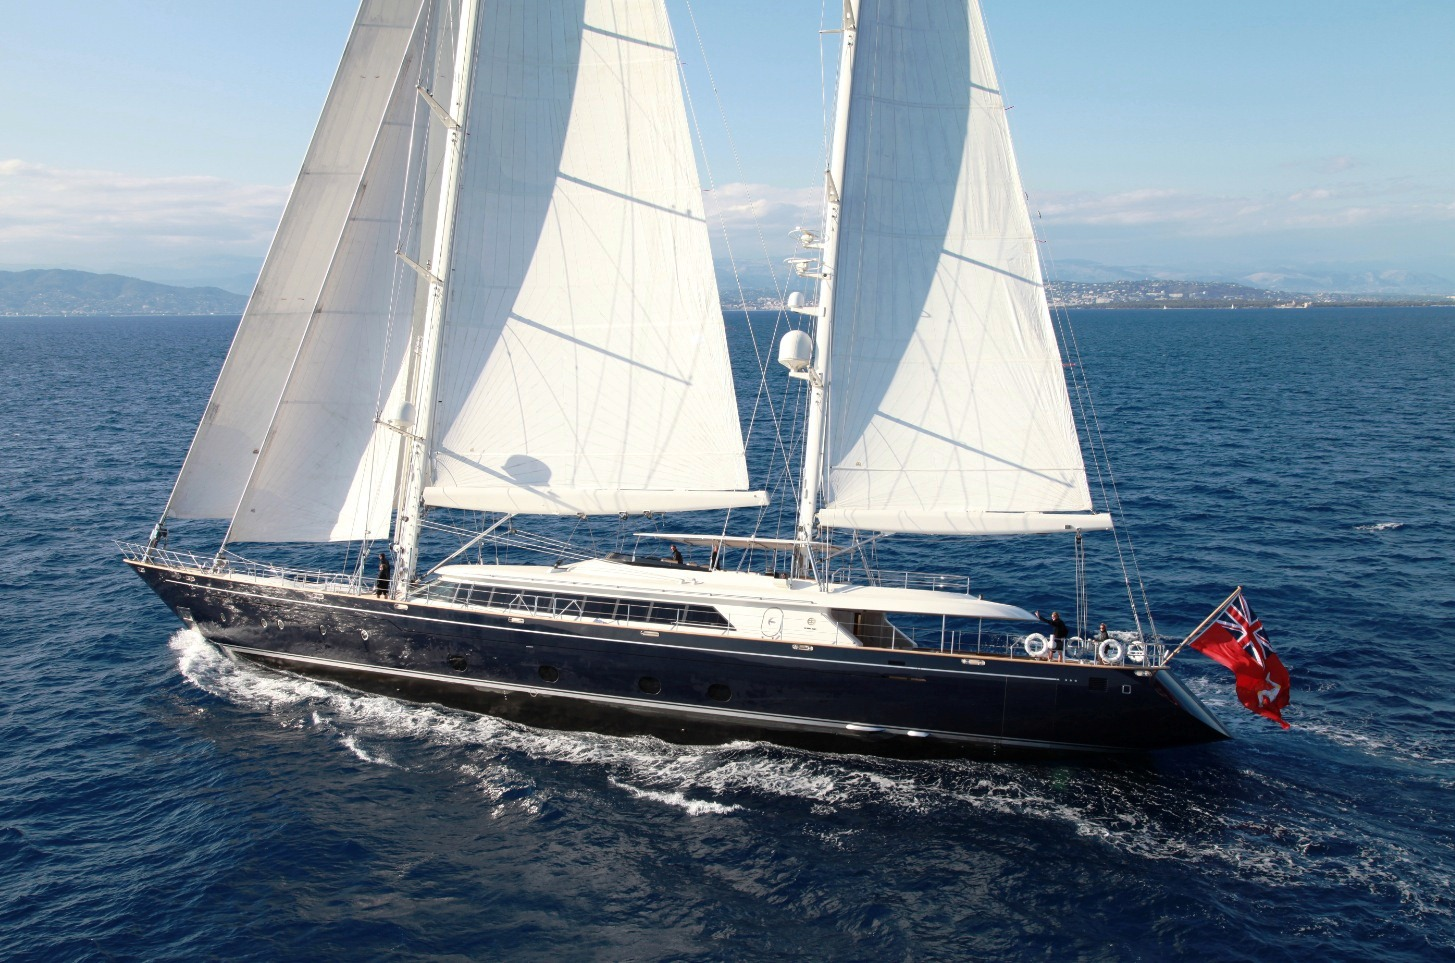
\includegraphics[width=\linewidth]{figs/boat.jpg}
  \caption{A boat.}
  \label{fig:boat1}
\end{figure}

As you can see Figure \ref{fig:boat1} shows a boat.

\subsection{Conclusion}

This should be enough to get you started. You just write in the Chapter files with these few basic commands, you will see that the root-file will include the individual chapter files in the US-thesis wrapper.
%\chapter{Literature Review}
\label{chp:litrev}


%%%%%%%%%%%%%%%%%%%%%%%%%%%%%%%%%%%%%%%%%%%%%%%%%%%%%%%%%%%%%%%%%%%%%%%
\section{Introduction}

Here you write your amazing text.
%\chapter{Chapter Title}
\label{chp:give-it-a-nice-label}


%%%%%%%%%%%%%%%%%%%%%%%%%%%%%%%%%%%%%%%%%%%%%%%%%%%%%%%%%%%%%%%%%%%%%%%
\section{Introduction}

Here you write your amazing text.
%\chapter{Chapter Title}
\label{chp:give-it-a-nice-label}


%%%%%%%%%%%%%%%%%%%%%%%%%%%%%%%%%%%%%%%%%%%%%%%%%%%%%%%%%%%%%%%%%%%%%%%
\section{Introduction}

Here you write your amazing text.
%\chapter{Chapter Title}
\label{chp:give-it-a-nice-label}


%%%%%%%%%%%%%%%%%%%%%%%%%%%%%%%%%%%%%%%%%%%%%%%%%%%%%%%%%%%%%%%%%%%%%%%
\section{Introduction}

Here you write your amazing text.
%
%%%...uncomment chapters as they get finished so that they are compiled.

%==== Appendices ====================================================
\appendix
\appendixpage\relax

\chapter{Research Instruments}
\label{chp:res-inst}

\section{Interview Guide}
\label{sec:int-guide}

Here you can include your interview guide
\subsection{SubSection}

It can have subsections too.

\section{Survey Instrument}

Then you can include your survey questions under a new heading too. Or you might make it another appendix. And yet another for your ethical clearance documents and institutional permissions.

%--------------------------------------------------------------------
\endinput

%\include{contents/App-2}
%\include{contents/App-3}

%==== Bibliography acro's & Index ===================================
\bibliography

%\bibliography{backmatter/USbib-sample} %ORIGINAL PACKAGE OPTION
\printbibliography[] %BIBER OPTION

\end{document}
